\documentclass[]{article}
\usepackage[english]{babel}
\usepackage[explicit]{titlesec}
\usepackage{graphicx}

%opening
\title{Distributed Systems: Java RMI report}
\author{Tobias De Locht, Dries De Backker}
\date{3 November, 2017}

\begin{document}

\maketitle

\section{Design decisions}
The set up of this project consists of 2 packages, the client and the rental server, reflecting the client-server nature of the application. Figure \ref{fig:class} shows the class diagram of the project. For real life applications we chose to include a web server so that the client can download the necessary implementation classes from there instead. This deployment is visualized in figure \ref{fig:dep}.
\\
When starting up the RentalServer, its main method creates a new NamingService object. This object is mainly responsible for registering car rental companies and looking up their objects by name. The main method then creates a new remotely accessible SessionManager object. This one is in charge of creation and bookkeeping of new sessions for clients as well as managers. As per the instructions, two types of sessions are available, each implemented as remote object class inheriting from its remote interface. These remote objects are returned by the sessionManager, which the client can find in the RMI registry by name, and offer the application's functionality to the requesting client. Figure \ref{fig:client} shows a sequence diagram for a session creation by the client.
\\
Manager sessions are more or less stateless while the reservation sessions are stateful. The reservation sessions are used by clients to check car availabilities and make or cancel reservations. In order to do this, the session records the tentative reservation quotes made by the clients. Managers sessions do not record any such data. The sequence diagram for making a reservation is shown in figure \ref{fig:reservation}.
\\
For the session objects no life cycle management was implemented at this time. This means the session for a specific client or manager is not removed after he closes his application. In real life this naturally won't do. One can solve this issue by having the rental server's main method running a procedure that loops over the sessions in order to detect sessions that have not been in use for some time, so that they can be removed.
 
\section{Remote objects}
There are 3 remote classes, each with its corresponding remote interface. The SessionManager, ReservationSession and MangerSession classes. The objects of these classes are remote so that the client can invoke remote methods on them. The SessionManager object is stored in the RMI registry, the two session objects are not. These objects are stored are created in the SessionManager object and returned to the client upon requesting one such session. All remote objects live on the rental server because their implementation requires data and methods from this server, and because conceptually, they belong to the server's functionality.
\\
Some objects need to be returned over the remote connection. For this to be possible, these classes need to be serialized. For example, the Reservation class is a return value in some of the client's methods and is thus a serialized class. The class diagram shows which of these classes are made to be serializable.  

\section{Synchronization}
With the current deployment in use, it is possible multiple clients are concurrently sending method requests to the server. These request are then executed in interleaving threads. This way some data can become inconsistent. To solve this problem some methods at the server are defined as synchronized. This will make it impossible for these methods to interleave their thread executions and execute sequential instead. The methods to made synchronized are in the CarRentalCompany and the NamingService class because the objects of these classes are the ones that offer public methods to possibly concurrently running sessions. This has the potential to become a bottleneck since no concurrent read or write behaviour is allowed.
\clearpage
\section{Diagrams}
{\begin{figure}[h]
		\caption{Class Diagram}
		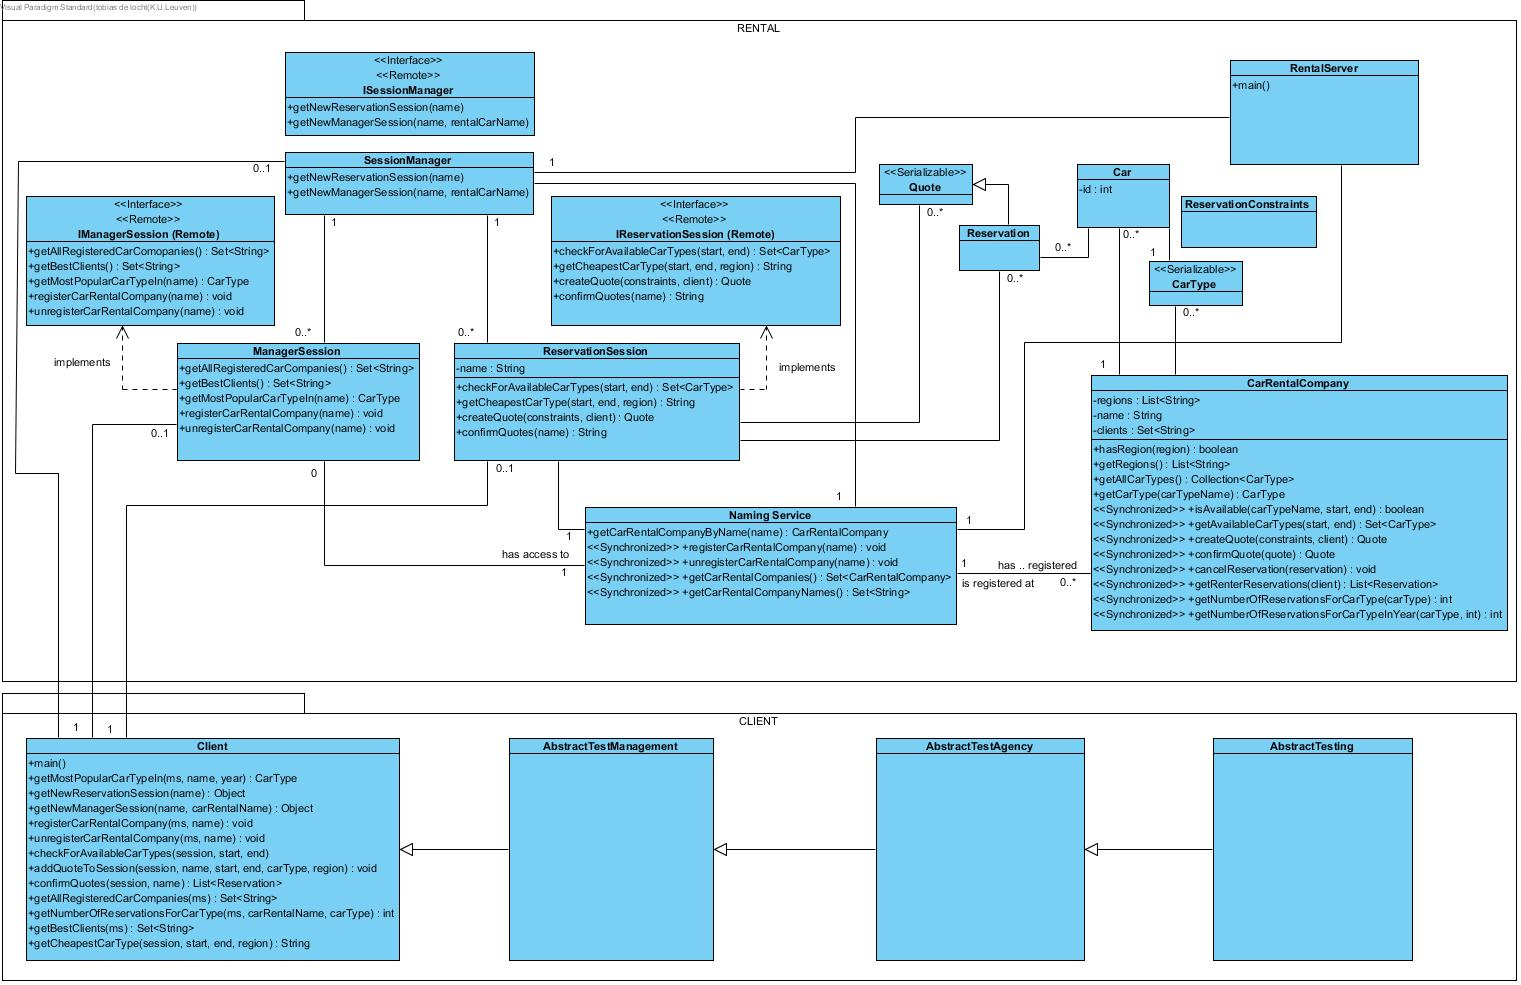
\includegraphics[width=1\textwidth]{classdiagram}
		\label{fig:class}
	\end{figure}
\clearpage
{\begin{figure}[h]
		\caption{Client session creation}
		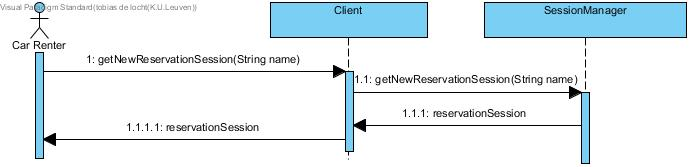
\includegraphics[width=1\textwidth]{clientseq}
		\label{fig:client}
	\end{figure}
{\begin{figure}[h]
		\caption{Reservation}
		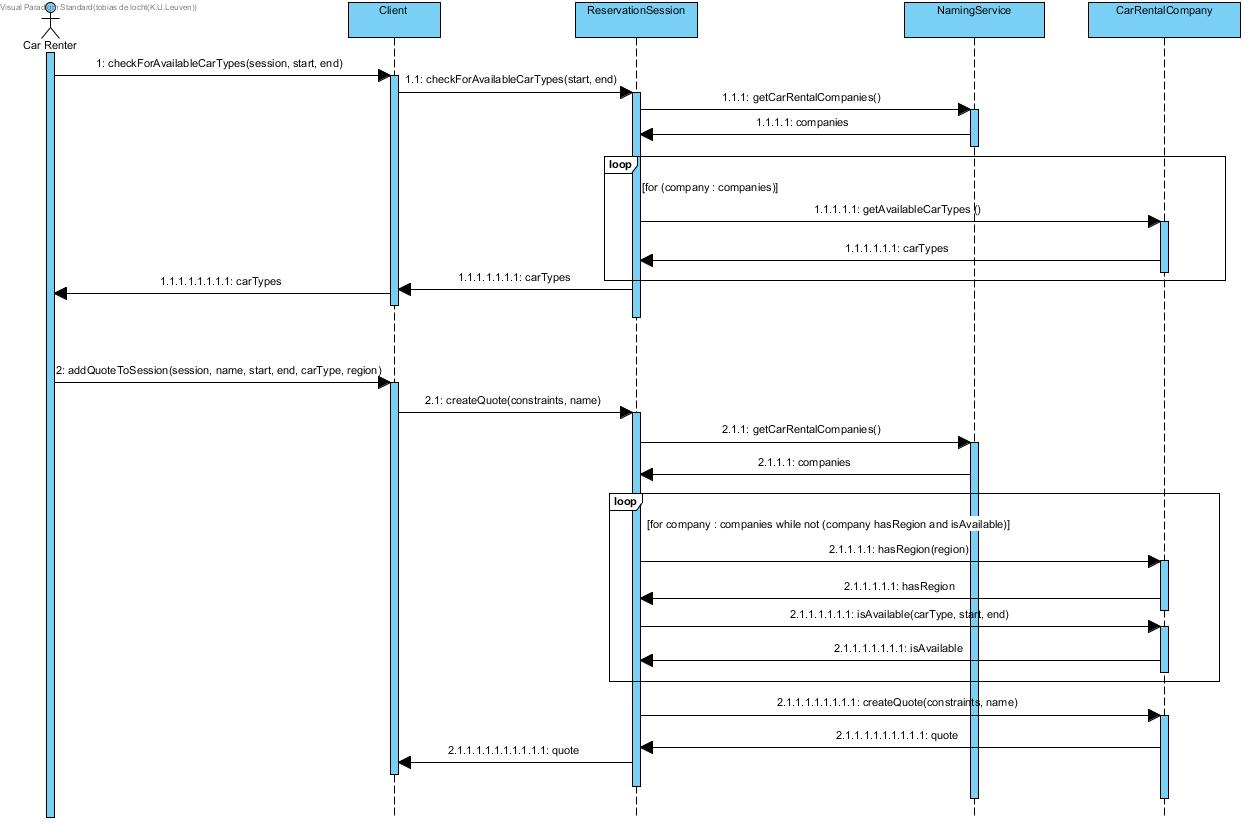
\includegraphics[width=1\textwidth]{reservationseq}
		\label{fig:reservation}
	\end{figure}
\clearpage
{\begin{figure}[h]
		\caption{Deployment}
		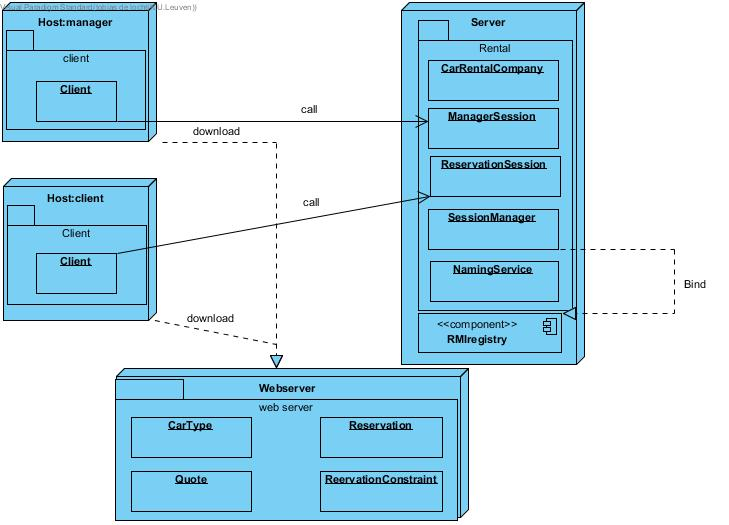
\includegraphics[width=1\textwidth]{deployment}
		\label{fig:dep}
	\end{figure}
\end{document}

